\documentclass{standalone}

\usepackage{tikz}
\usepackage{graphicx}
\pagestyle{empty}

% INT_AY22_L35-Fig02_Wire_approx.png

\begin{document}
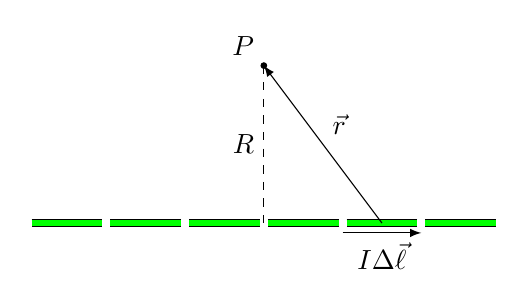
\begin{tikzpicture}[> = latex]

	% Definitions
	
	\def\L{6}		% Wire length
	\def\N{6} 		% Number of wire segments
	\def\R{2}		% Distance to observation point
	
	% Wire segments
	
	\foreach \n in {0, 1, ..., 5}
		\draw [double = green, double distance = 2 pt] ({(\n + 0.05) * \L / \N}, 0) -- ({(\n + 0.95) * \L / \N}, 0);
		
	% Observation point P
	
	\filldraw (0.5 * \L, \R) circle (1 pt) node [above left] {$P$};
	\draw [dashed] (0.5 * \L, \R) -- node [left] {$R$} (0.5 * \L, 0);
		
	% Radius vector
	
	\draw [->] ({(\N - 1.5) * \L / \N}, 0) -- node [above right] {${\vec r}$} (0.5 * \L, 2);
	
	% Length vector
	
	\draw [->] ({(\N - 2) * \L / \N}, -0.125) -- node [below] {$I \Delta {\vec \ell}$} ({(\N - 1) * \L / \N}, -0.125);

\end{tikzpicture}
\end{document}